\section{Disponibilidade do METAR}

Durante as enchentes de grandes proporções no Rio Grande do Sul ocorridas em maio de 2024, grande
parte da capital Porto Alegre ficou alagada. O Aeroporto Internacional Salgado Filho fechou, já
que grande parte do pátio e da pista ficaram debaixo de água, impossibilitando pousos e decolagens.
Algumas aeronaves particulares foram danificadas pela água.

Com o aeroporto fechado, o METAR não era mais emitido. Porém, a API do Aviation Weather não
respondia com um código HTTP de erro ou de não encontrado, mas sim com código 200 e uma string
vazia como resposta. Para o aeroporto, a seguinte tela aparecia:

\begin{figure}[ht]
    \begin{center}
    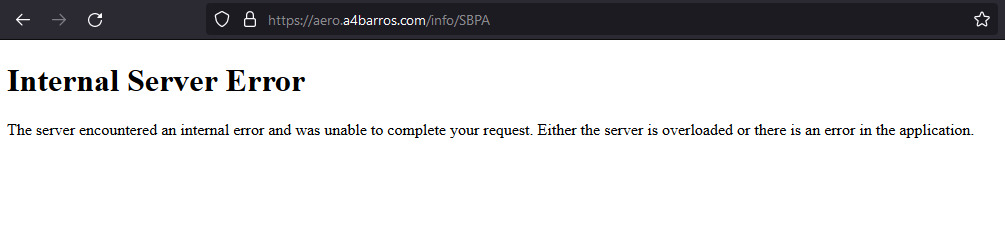
\includegraphics[width=400pt]{img/sbpa-erro.png}
    \caption{Página com o erro}
    \label{fig:sbpa-erro}
    \end{center}
\end{figure}

Quando o módulo de decodificação do METAR tentava buscar o dia e hora na string do METAR, esta
não existia. Então, quando tentava buscar certo índice no resultado do regex, o resultado era None.
Então a exceção ValueError era levantada.

Já que todo METAR deve possuir o item com o dia e a hora zulu, caso este não exista, a função de
decodificação do METAR retorna uma mensagem de METAR indisponível.

\begin{figure}[ht]
    \begin{center}
    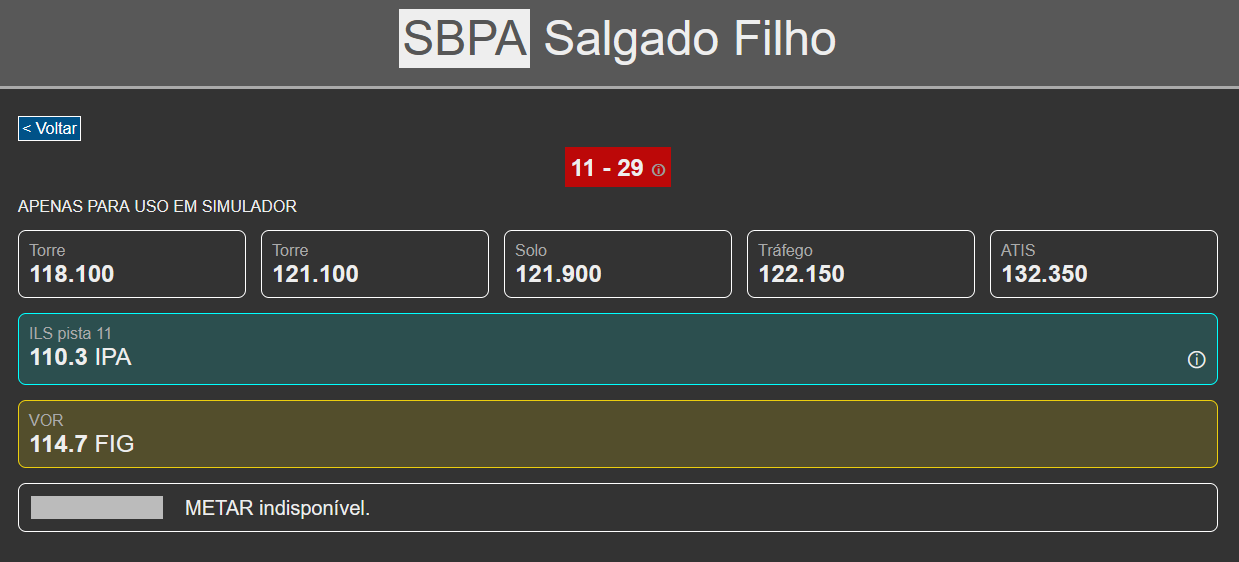
\includegraphics[width=400pt]{img/sbpa.png}
    \caption{Página com o fallback}
    \label{fig:sbpa}
    \end{center}
\end{figure}
